%\section{Proposed Model}
\section{Proposed Model} 
We will use Deep Learning in our work which is a BlackBox function. Generally, Black boxes work excellently but their structure won’t give you any insights that will explain how the function is being approximated. For this, we will use LIME which is one of the most popular XAI-based python libraries. There are a lot of XAI frameworks that explain the BlackBox model’s insights by features. XAI functions work well in terms of explaining complex classification models. In short, these functions generate an explanation through charts of graphs for a complex model's prediction which are also pretty fast. In Figure 4.1 we will see how black boxes work.

\vspace{5mm}
\begin{figure}[htbp]
\centering
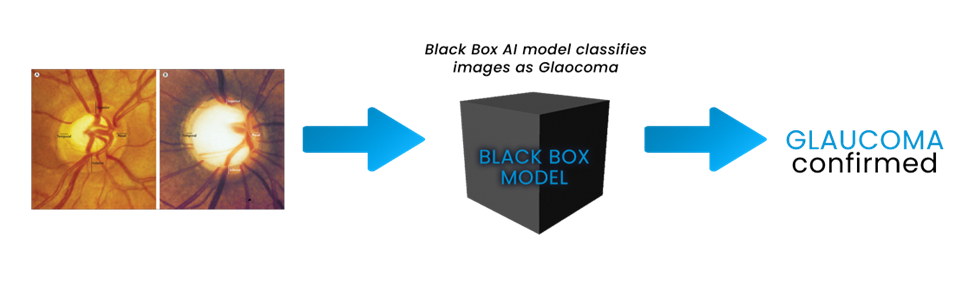
\includegraphics[scale=0.70]{images/fig-1.png}
\caption{Blackbox models confirming glaucoma through images}
\label{fig:x Blackbox models confirming glaucoma through images}
\end{figure}

\vspace{5mm}
In Figure 4.2 we will see how black boxes actually work with the help of lime.

\vspace{5mm}
\begin{figure}[htbp]
\centering
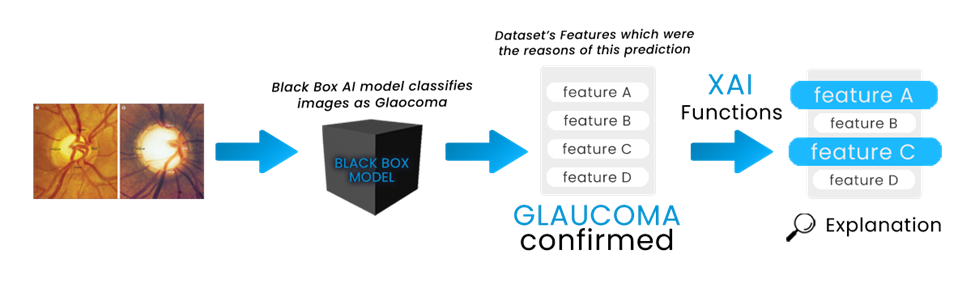
\includegraphics[scale=0.70]{images/fig-2.png}
\caption{Blackbox models decision making explanation through LIME}
\label{fig:x Blackbox models decision making explanation through LIME}
\end{figure}

\vspace{5mm}
\noindent Here we can see BlackBox models generate a result or output based on some features from the given/training datasets. And through lime, we can have a visualization from which features the output was based on.

\vspace{5mm}
\noindent In our Glaucoma dataset, we have some features for Suspicious glaucoma and Non-glaucoma. In both sections, we have \textbf{attention map}, \textbf{images}, and \textbf{labels} as \textbf{1} as the confirmed glaucoma case and \textbf{0} as the Non-glaucoma case. To apply XAI, we took \textbf{Convolutional Neural Network (CNN)}, \textbf{Support Vector Machine (SVM)}, \textbf{Fully Connected Neural Network (FCNNs)} as a black box AI model to predict glaucoma with the help of the data. To compile all of these classifications and determine the average of these scores to one single output, we will use the Softmax function. Below a short rendition is being given for the above Deep Learning models.

\vspace{5mm}
\noindent 1.    \textbf{Convolutional Neural Network (CNN)}: In deep learning, a convolutional neural network (CNN, or ConvNet) is a class of deep neural networks, most commonly applied to analyze visual imagery. We will classify the image data through this model.

\vspace{5mm}
\noindent 2.    \textbf{Support Vector Machine (SVM)}: SVM is a supervised machine learning classifier that may be used to categorize or to regression problems.
It uses a method called the kernel trick to transform your data and then calculates an appropriate boundary between various outputs based on these modifications. With this model, we will get a predicted output.

\vspace{5mm}
\noindent 3.    \textbf{Fully Connected Neural Network (FCNNs)}: Fully connected neural networks (FCNNs) are a type of artificial neural network where the architecture is such that all the nodes, or neurons, are in one layer, are connected to the neurons in the next layer [22]. This model will also help us to predict and output.

\vspace{5mm}
\noindent 4.    \textbf{Softmax}: Softmax is a mathematical function that transforms a vector of integers into a vector of probabilities, with the probability of each value proportional to the vector's relative scale. The softmax function is most commonly used as an activation function in a neural network model in applied machine learning. The network is set up to produce N values, one for each classification task class, and the softmax function is used to normalize the outputs, turning them from weighted sum values to probabilities that total to one. Each value in the output of the softmax function is interpreted as the probability of membership for each class. This will compile the outputs of SVM and FCNNs into a single output.

\newpage
\section{Work Plan} 
According to our Dataset, we will divide the data in a ratio of 8:2 chronologically training and testing data to classify glaucoma with the help above deep learning models. And through any XAI function, we will explain these black boxes.

\begin{figure}[htbp]
\centering
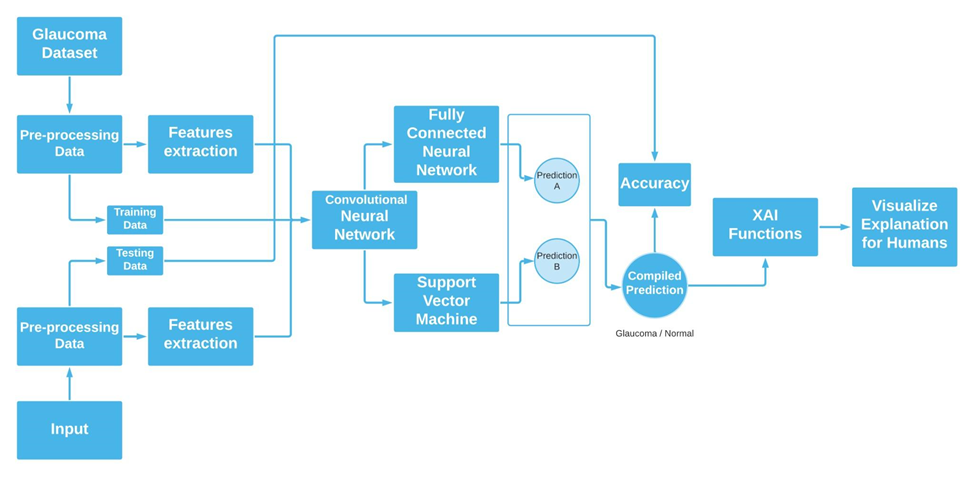
\includegraphics[scale=0.75]{images/fig-3.png}
\caption{Work plan of the whole project}
\label{fig:x Work plan of the whole project}
\end{figure}

\vspace{5mm}
\noindent Here in [Figure 4.3], we have shown the whole process from dataset preprocessing to compiled output through Softmax. And with XAI functions, we will explain the black boxes through visualization charts of the used core features which were the main reasons behind the prediction.